%-*- coding: UTF-8 -*-
% gng_spec.tex
% Gaussian Noise Generator Core Specification

\documentclass[a4paper, titlepage]{article}

\usepackage{amsmath}
\usepackage[no-math]{fontspec}
\usepackage{unicode-math}
\usepackage[nottoc]{tocbibind}
\usepackage{siunitx}
\usepackage{xcolor}
\usepackage{graphicx}
\usepackage{booktabs}
\usepackage{hyperref}

\setmainfont{Minion Pro}
\setsansfont{Myriad Pro}
\setmonofont{Consolas}
\setmathfont{XITS Math}[math-style=ISO]

\pagestyle{headings}
\renewcommand{\thepage}{\oldstylenums{\arabic{page}}}

\hypersetup{colorlinks,%
    linkcolor=cyan!30!black, citecolor=green!50!black,%
    urlcolor=magenta!50!black,%
    pdfstartview=FitH}

\DeclareMathOperator{\ICDF}{ICDF}
\DeclareMathOperator{\erf}{erf}

\graphicspath{{figures/}}

\bibliographystyle{plain}


\begin{document}

% Title page
\begin{titlepage}
\begin{flushleft}
    \normalfont
    {\bfseries\fontsize{32pt}{32pt}\selectfont
    Gaussian Noise Generator}

    \vspace{4ex}
    {\bfseries\fontsize{24pt}{24pt}\selectfont
    IP Core Specification}

    \vspace{20ex}
    {\LARGE\bfseries Guangxi Liu}

    \medskip
    {\Large\itshape guangxi.liu@opencores.org}
\end{flushleft}

\vspace*{\fill}

\begin{flushright}
{\Large Revision \oldstylenums{1.1}}

\medskip
{\Large \oldstylenums{\today}}
\end{flushright}
\end{titlepage}


% Table of contents
\tableofcontents
\clearpage


% Main parts
\section{Introduction}

\subsection{Description}
The \emph{Gaussian Noise Generator} (GNG) core generates white Gaussian noise of
standard normal distribution, which can be used to measure BER to
extremely low BER levels (\num{e-15}).
The core uses a 64-bit combined Tausworthe generator and an approximation of
the inverse normal cumulative distribution function,
which obtains a PDF that is Gaussian to up to 9.1$\sigma$.
The core was designed using synthesizable Verilog code and can be delivered as
a soft-IP targeted for any FPGA device and ASIC technology.
C/MATLAB models and corresponding test benches are also available.

\subsection{Features}
\begin{itemize}
    \item Period of generated noise sequence is about \si{\raiseto{176}2}
    \item Random distribution in the range of $\pm$9.1$\sigma$
    \item Noise is quantized to 16 bits with 5 bits of integer
        and 11 bits of fraction
    \item Internal 64-bit uniform random number generator with
        configurable initial seeds
    \item Based on a piecewise polynomial approximation of
        the inverse normal cumulative distribution function
    \item High throughput, over 300 MHz clock rate and
        output sample rate in advanced FPGA
    \item Fully synchronous design using single clock
    \item Design optimized for Xilinx \& Altera FPGA technology
\end{itemize}

\subsection{Applications}
\begin{itemize}
    \item Communication system requiring accurate emulation of an AWGN channel
    \item Bit error rate measurement system
\end{itemize}


\section{Algorithm}

\subsection{Overview}
Most digital methods for generating Gaussian random variables are
based on the transformation of uniformly distributed random variables.
The most important methods for the design of hardware GNG are summarized below.

\subsubsection{CLT}
The central limit theorem (CLT) states that the sum of
a sufficiently large number of independent uniformly
distributed random variables will be approximately normally distributed.
High accuracy GNGs need to sum up a large number of samples and
the CLT method is not suitable for high-speed applications.

\subsubsection{B-M Method}
The Box–Muller (B-M) method has been widely used to generate
Gaussian noise samples.
This method is based on the transformation of two independent uniformly
distributed random numbers, i.e., $\mathrm{U}(0,1)$,
using elementary functions (sqrt, ln, and cos/sin).

\subsubsection{Rejection–Acceptance Methods}
The rejection–acceptance methods, basically the Polar method and
the Ziggurat method, are the most important methods in
software random number generation.
Their main drawback is the use of conditional statements that
lead to a nonconstant output rate.

\subsubsection{Wallace Method}
The Wallace method is based on the fact that linear combinations of
Gaussian-distributed random numbers are also Gaussian distributed.
This method avoids the evaluation of transcendental functions.

\subsubsection{ICDF}
The inversion method is based on the use of the ICDF of
the Gaussian distribution to transform a uniformly distributed random
variable $x$ into a Gaussian variable $y$ through $y = \ICDF(x)$.
Using this method, it is possible to generate random samples for
arbitrary distributions.
This method is used as the design presented here.

\subsection{CTG}
Although traditional linear feedback shift registers (LFSRs) are often
sufficient as a uniform random number generator (URNG),
Tausworthe URNGs are fast and occupy less area.
Furthermore, they provide superior randomness when
evaluated using the Diehard random number test suite.

The combined Tausworthe generator (CTG) is used here follows the algorithm
presented by \cite{lecuyer1}, \cite{lecuyer2},
which generates a 64-bit uniform random number per clock
and has a large period of \si{\raiseto{176}2}($\approx$\num{e53}).
The parameters of generator are as follows (see Table 2 in \cite{lecuyer2}):
\begin{align}
    L = 64, J &= 3, k = 176; \\
    (k1, k2, k3) &= (63, 58, 55); \\
    (q1, q2, q3) &= (5, 19, 24); \\
    (s1, s2, s3) &= (24, 13, 7).
\end{align}

The algorithm is described in \cite{lecuyer1}, and special process is used
in generating valid initial state of generator.
See relative codes of design.

\subsection{ICDF}
The inversion method generates Gaussian samples via the ICDF of
the Gaussian distribution.
A uniformly distributed random sample $x \in \mathrm{U}(0,1)$ is
transformed into a sample y with the desired
probability density function applying $y = \ICDF(x)$.
The definition of ICDF is
\begin{equation}
    \ICDF(x) = \sqrt{2}\erf^{-1}(2x-1).
\end{equation}
The curve of it is shown in Figure \ref{fig:icdfplot}.
\begin{figure}[!htbp]
\centering
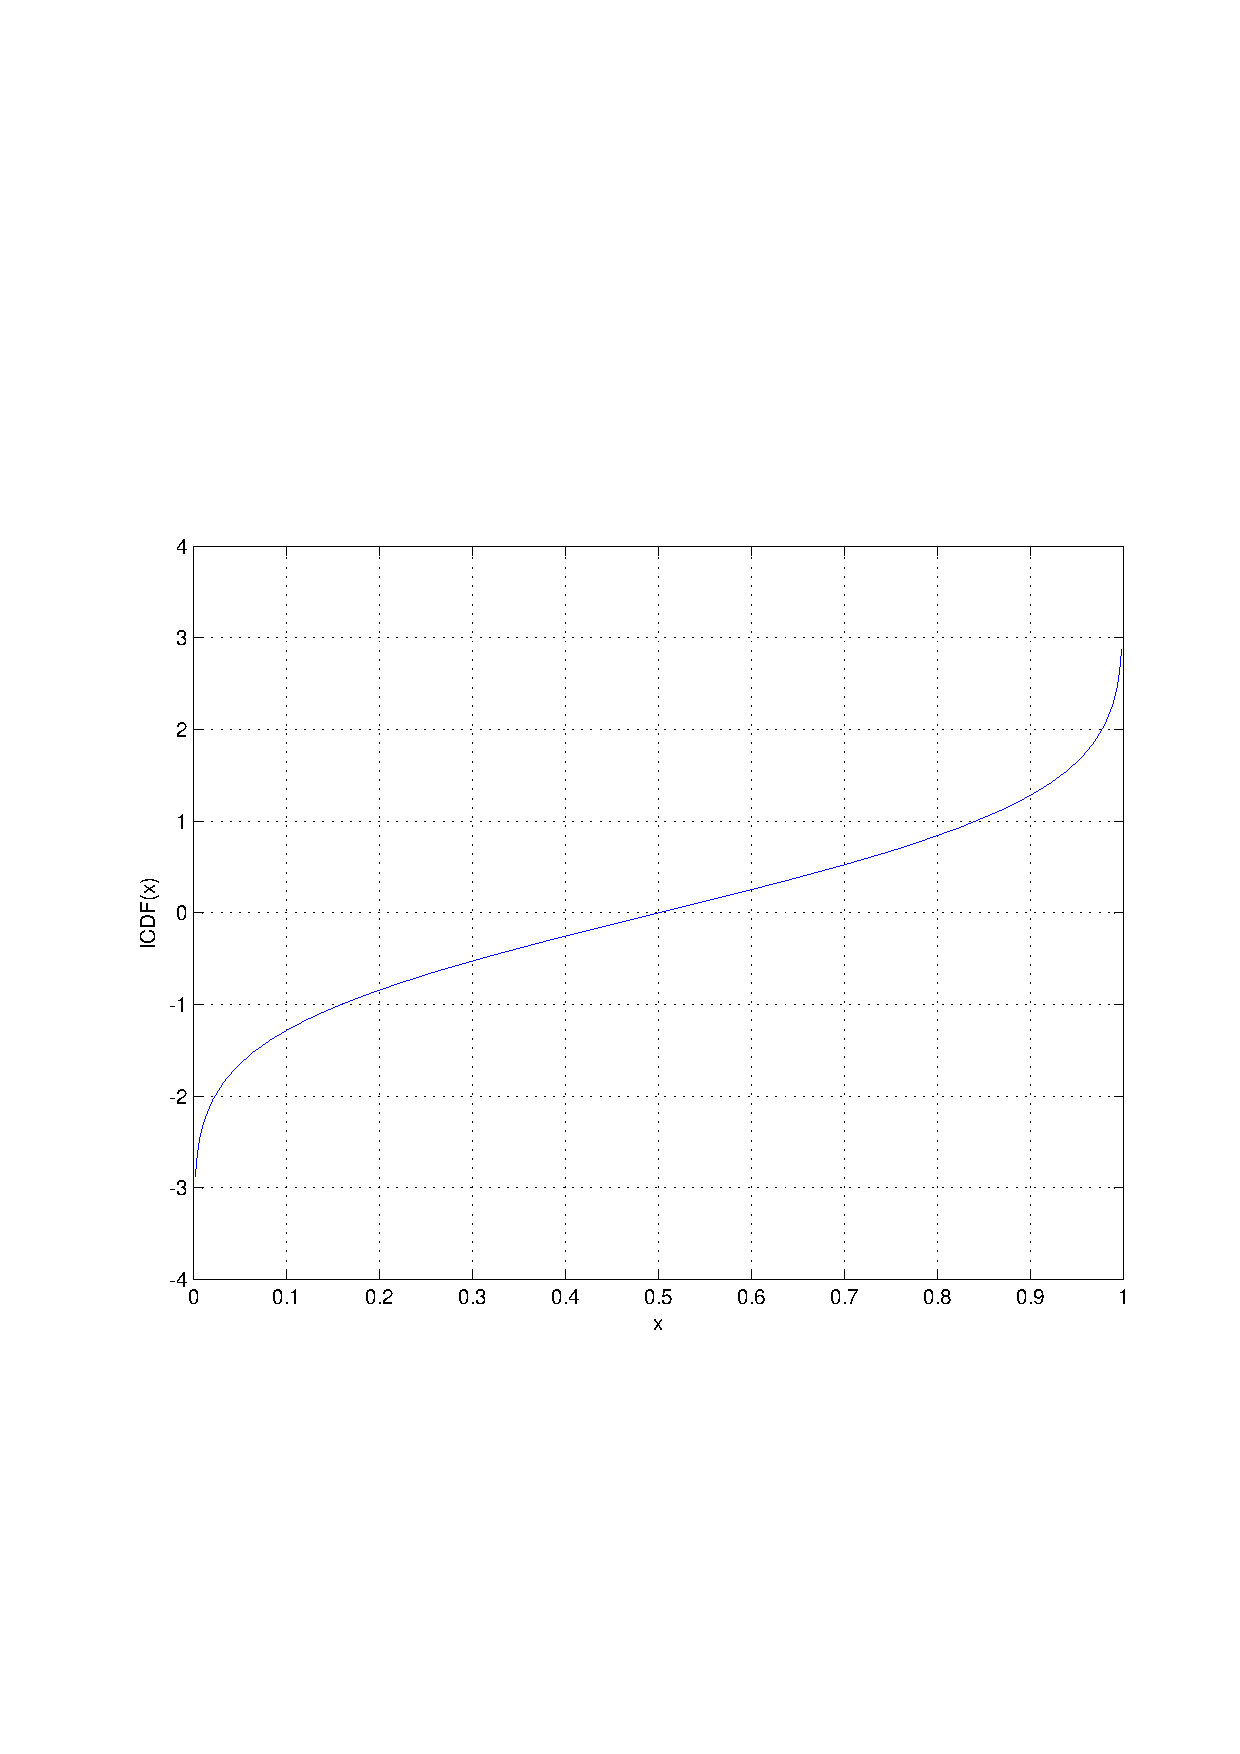
\includegraphics[width=0.85\textwidth]{icdfplot.pdf}
\caption{Curve of function ICDF(x).}
\label{fig:icdfplot}
\end{figure}

It is highly nonlinear when x approaches 0 or 1.
Besides, the curve is center symmetric with $x = 0.5$.
So only the part of $x > 0.5$ is considered except sign.

The design uses a nonuniform segmentation scheme
for the ICDF approximation.
Typically, the most significant bits (MSBs) of the URNG output
determine the segment and from the rest of the bits,
the most significant ones are used as the input for
interpolation inside the selected segment.
So, we need to compute $\ICDF(u)$, $u$ being the value obtained
if the bits of the URNG output are interpreted as
an unsigned binary representation (64 bits here).

The architecture of nonuniform segmentation scheme for
the ICDF approximation is similar to the one proposed in \cite{cheung} for
the hierarchical segmentation.
The segmentation of the function leads to two basic blocks in
the ICDF computation: segment selection and
interpolation inside the selected segment.
For interval (0, 0.5], $\mathrm{P2S_L}$ segmentation schemes is used for
the first pass and then $\mathrm{US}$ for the second pass.

The hardware computes $\ICDF(u')$, $u'$ being another uniform variable,
which is different from $u$, created also from the URNG output bits.
$\ICDF(u')$ can be computed more efficiently than $\ICDF(u)$,
both being uniformly distributed variables with the same word length and,
therefore, leading to the same output precision \cite{gutierrez}.

For each inner segment, a second order polynomial evaluation is performed,
that is
\begin{equation}
    y = (C_2x + C_1)x + C_0.
\end{equation}
And we need to find the best coefficients $C_0$, $C_1$ and $C_2$
making the approximation error minimum.
For real hardware implementation, these coefficients required
further converted to fixed-point.

\subsection{Performance}
The error plot of each segment is shown in Figure \ref{fig:errplot}.
For each segment, only the maximum error between
fixed-point and ideal result is shown.
\begin{figure}[!htbp]
\centering
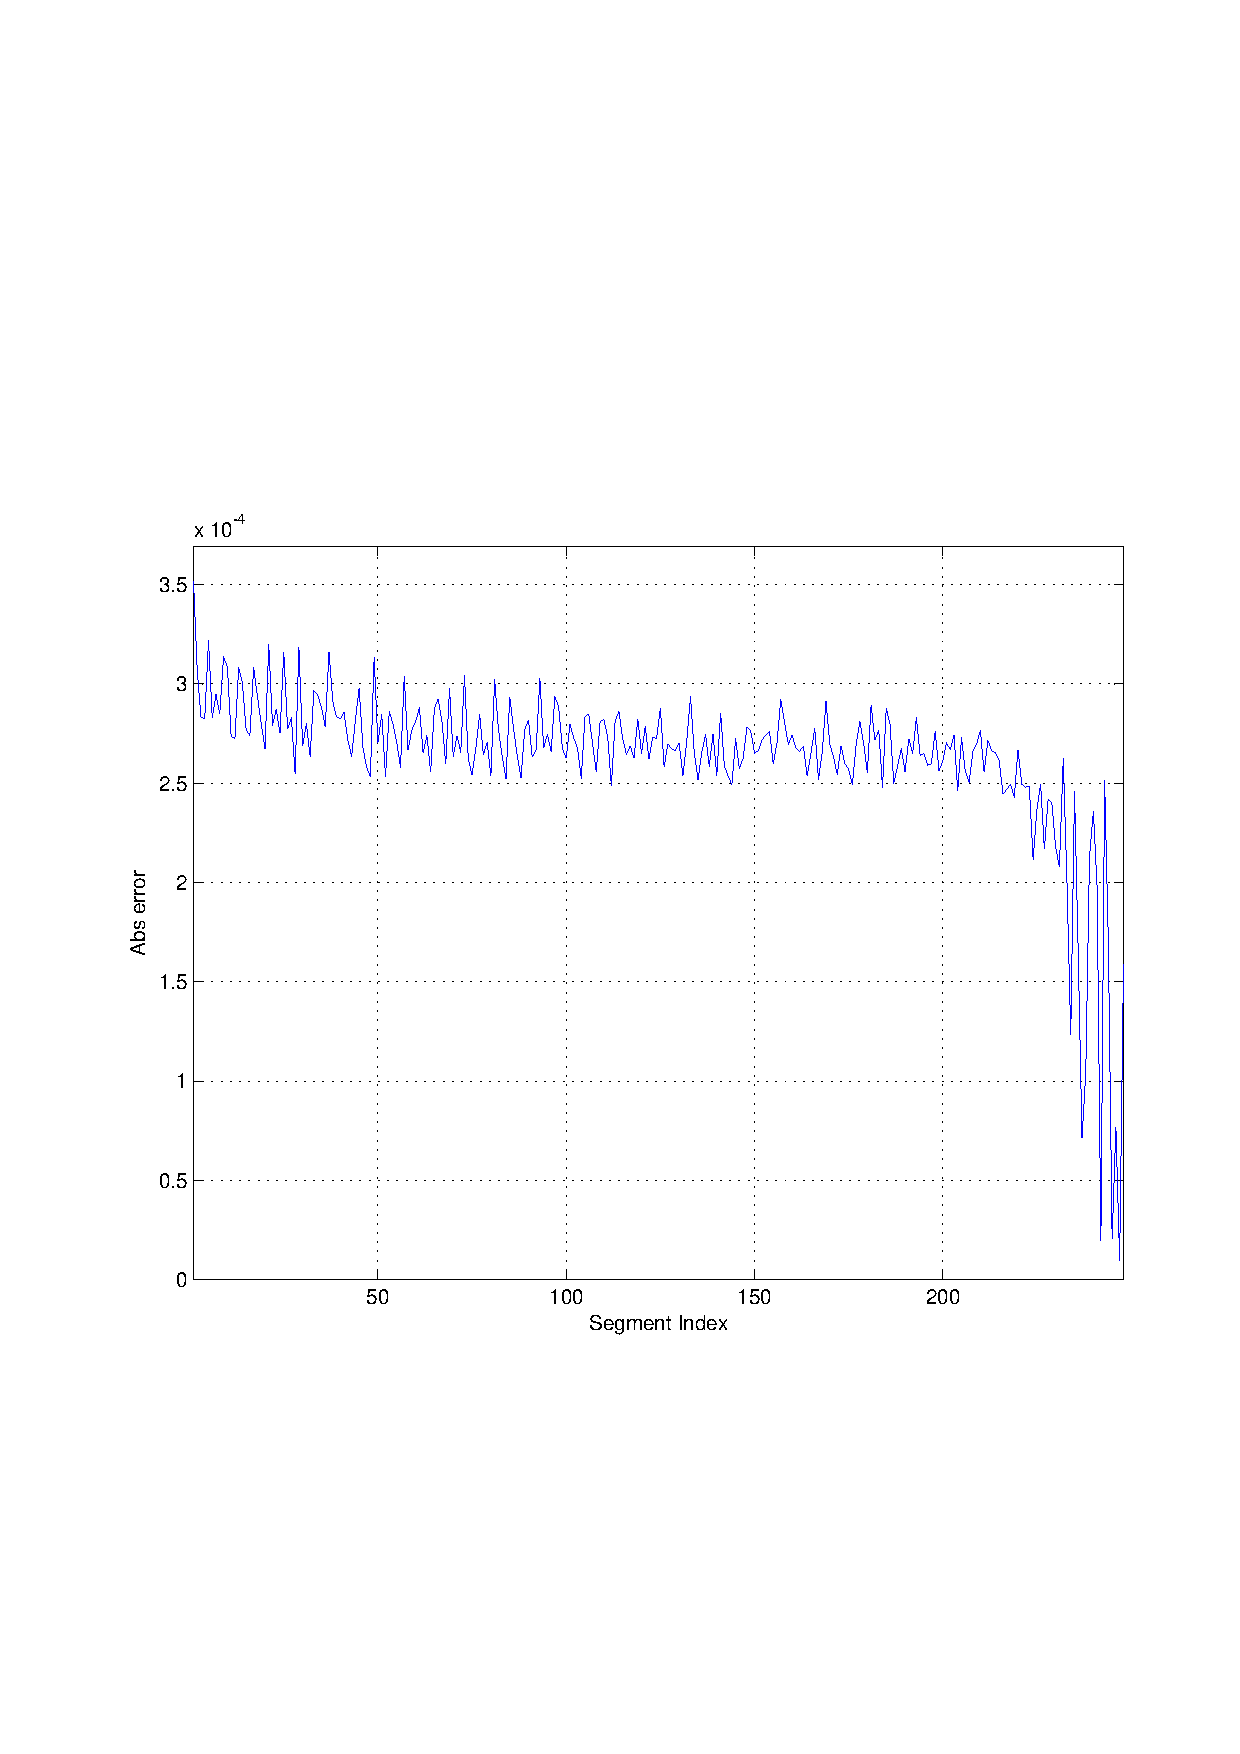
\includegraphics[width=0.85\textwidth]{errplot.pdf}
\caption{Error plot for each segment.}
\label{fig:errplot}
\end{figure}

From above plot, the maximum absolute error is about \num{0.00035},
which is about 0.72 ulp (1 ulp = \si{\raiseto{-11}2}).
The result satisfies system accuracy requirement.

Figure \ref{fig:pdfplot} below shows the PDF of generated samples for
a population of 10 million.
The black solid line indicates the ideal Gaussian PDF.
We can see that the generated samples closely follow the true Gaussian PDF.
\begin{figure}[!htbp]
\centering
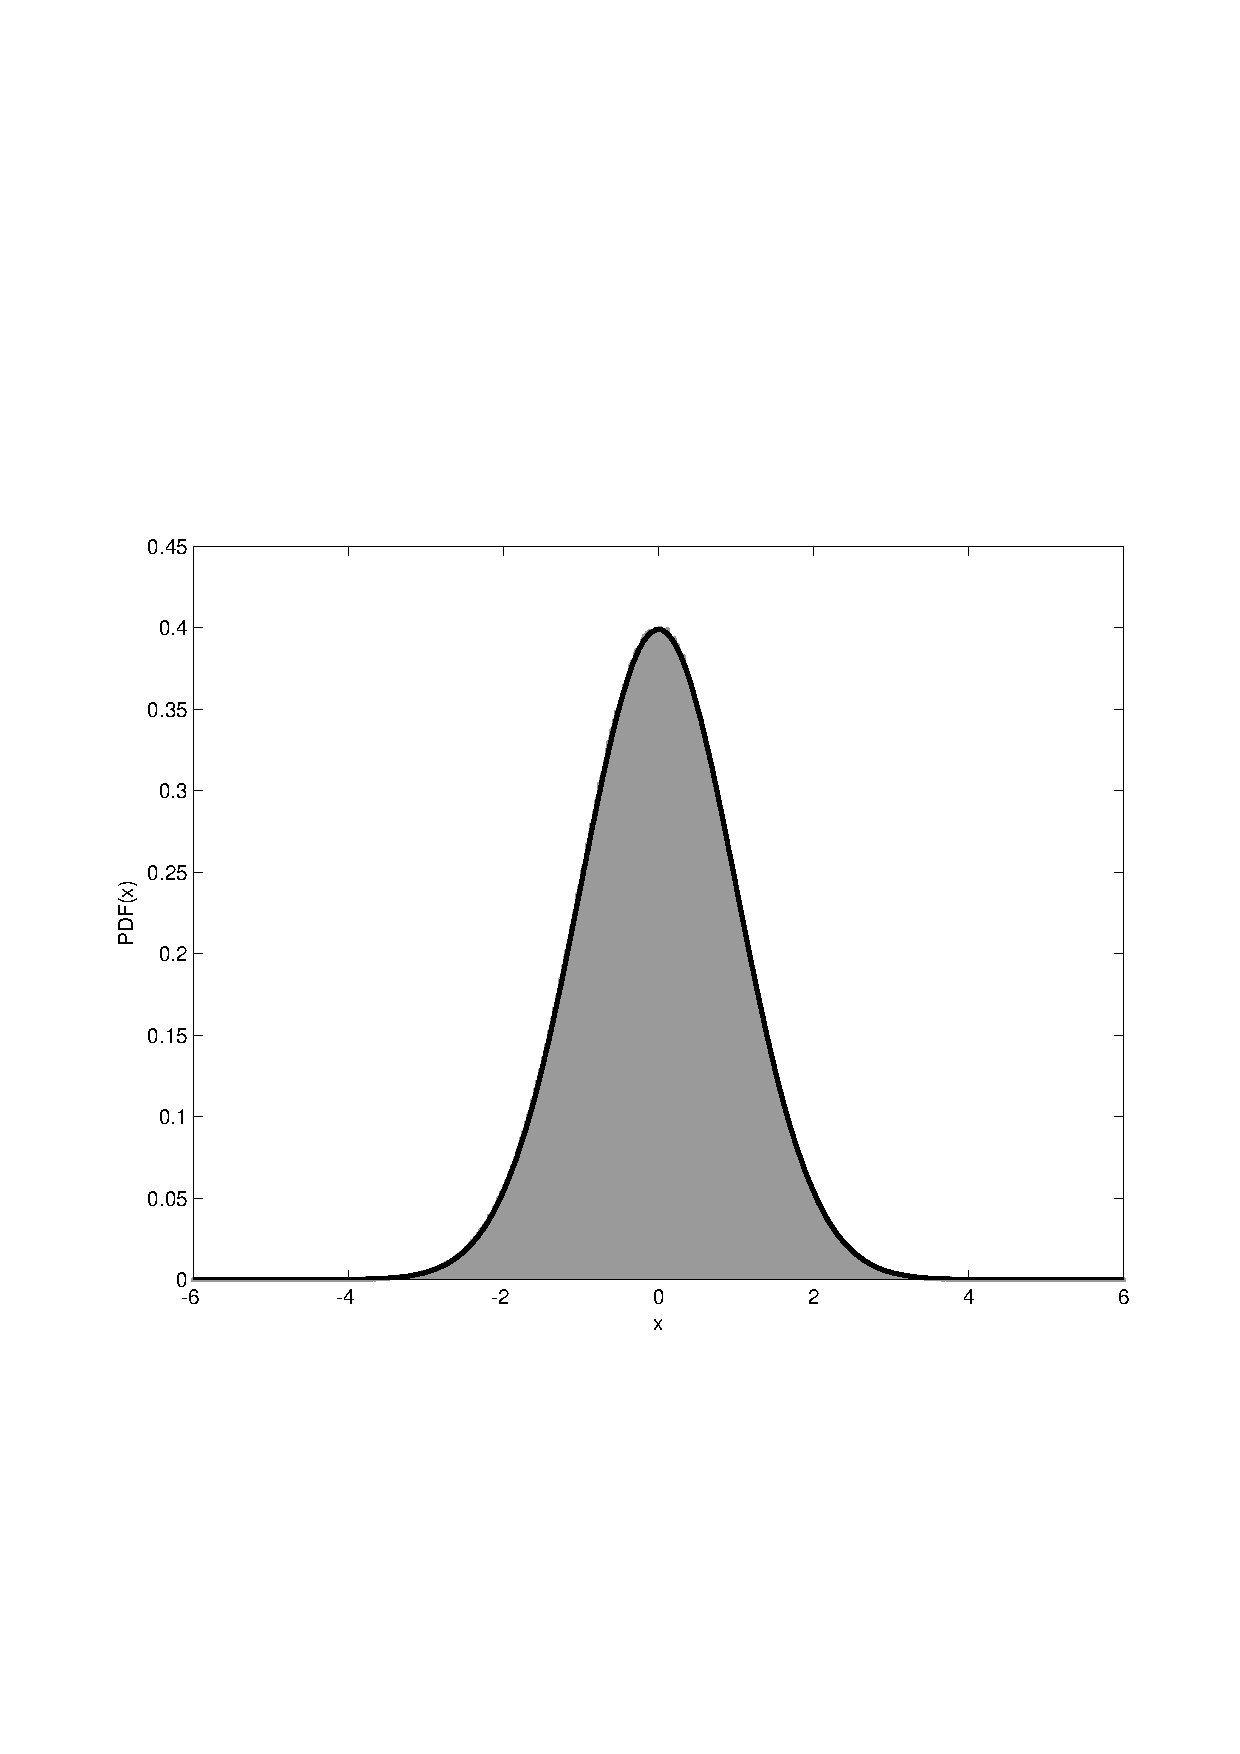
\includegraphics[width=0.85\textwidth]{pdfplot.pdf}
\caption{PDF of the generated samples for 10 million samples.}
\label{fig:pdfplot}
\end{figure}


\section{Implementation}

\subsection{Schematic Symbol}
The schematic symbol for the core is shown in Figure \ref{fig:coresch}.
\begin{figure}[!htbp]
\centering
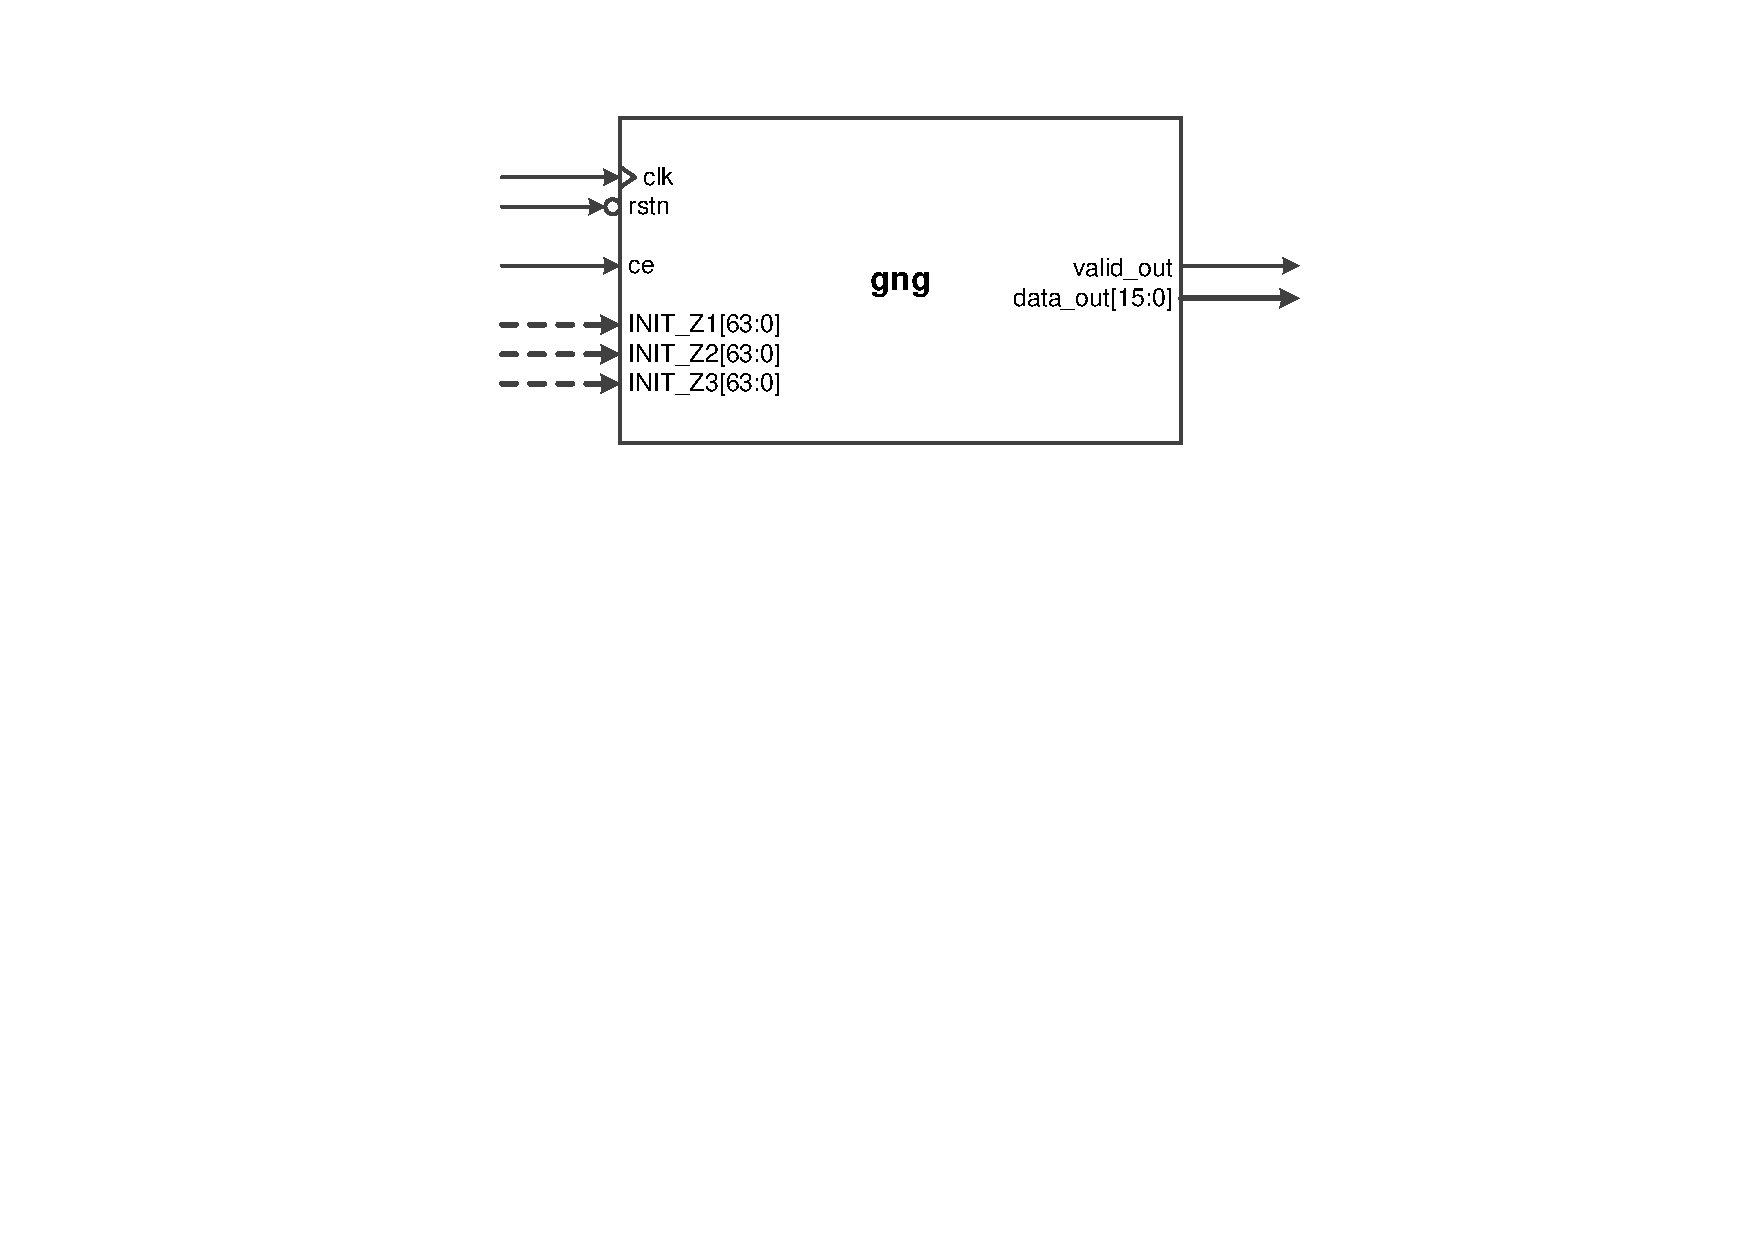
\includegraphics[scale=0.7,angle=270]{coresch.pdf}
\caption{Core schematic symbol.}
\label{fig:coresch}
\end{figure}

\subsection{Parameters}
The parameters for the core are shown in Table \ref{tbl:coreparam}.
\begin{table}[!htbp]
\centering
\caption{Core parameters.}
\label{tbl:coreparam}
\begin{tabular}{ccl}
    \addlinespace
    \toprule

    \textbf{Name} & \textbf{Width} & \textbf{Description} \\

    \midrule

    \textsf{INIT\_Z1} & 64 & Initial state value for CTG sub module 1 \\
    \textsf{INIT\_Z2} & 64 & Initial state value for CTG sub module 2 \\
    \textsf{INIT\_Z3} & 64 & Initial state value for CTG sub module 3 \\

    \bottomrule
\end{tabular}
\end{table}

\subsection{Ports}
The ports for the core are shown in Table \ref{tbl:coreport}.
\begin{table}[!htbp]
\centering
\caption{Core ports.}
\label{tbl:coreport}
\begin{tabular}{cccl}
    \addlinespace
    \toprule

    \textbf{Name} & \textbf{Width} & \textbf{Direction} & \textbf{Description} \\

    \midrule

    \textsf{clk} & 1 & Input & System clock \\
    \textsf{rstn} & 1 & Input & System synchronous reset, active low \\
    \textsf{ce} & 1 & Input & Clock enable \\
    \textsf{valid\_out} & 1 & Output & Output data valid \\
    \textsf{data\_out} & 16 & Output & Output data, fixed point format s<16,11> \\

    \bottomrule
\end{tabular}
\end{table}

\subsection{Structure}
\subsubsection{Top Module}
The top module comprises module \textsf{CTG} and \textsf{ICDF},
as shown in Figure \ref{fig:topmodule}.
\begin{figure}[!htbp]
\centering
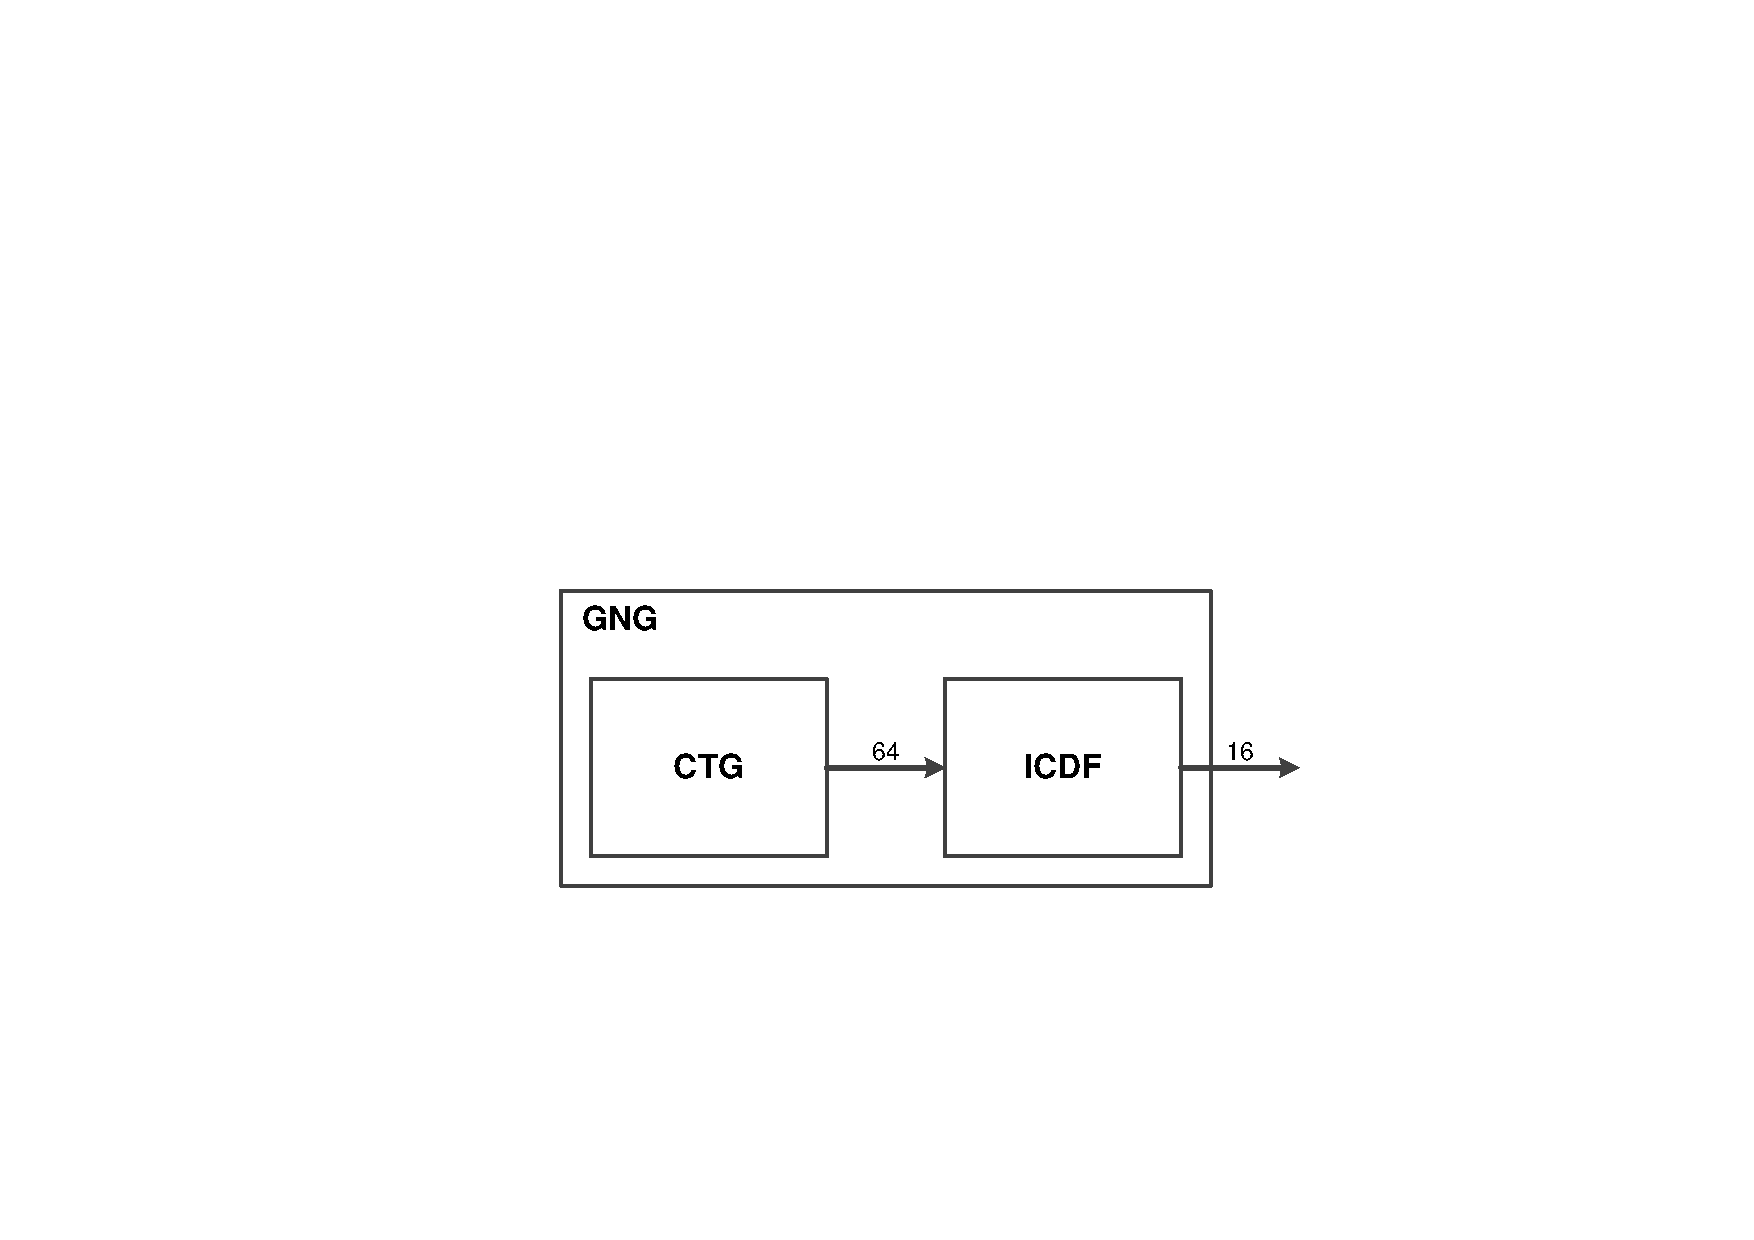
\includegraphics[scale=0.7,angle=270]{topmodule.pdf}
\caption{Top module architecture.}
\label{fig:topmodule}
\end{figure}

\subsubsection{CTG}
The architecture of \textsf{CTG} is depicted in Figure \ref{fig:ctgarch}.
For simplicity the control signals are not presented.
\begin{figure}[!htbp]
\centering
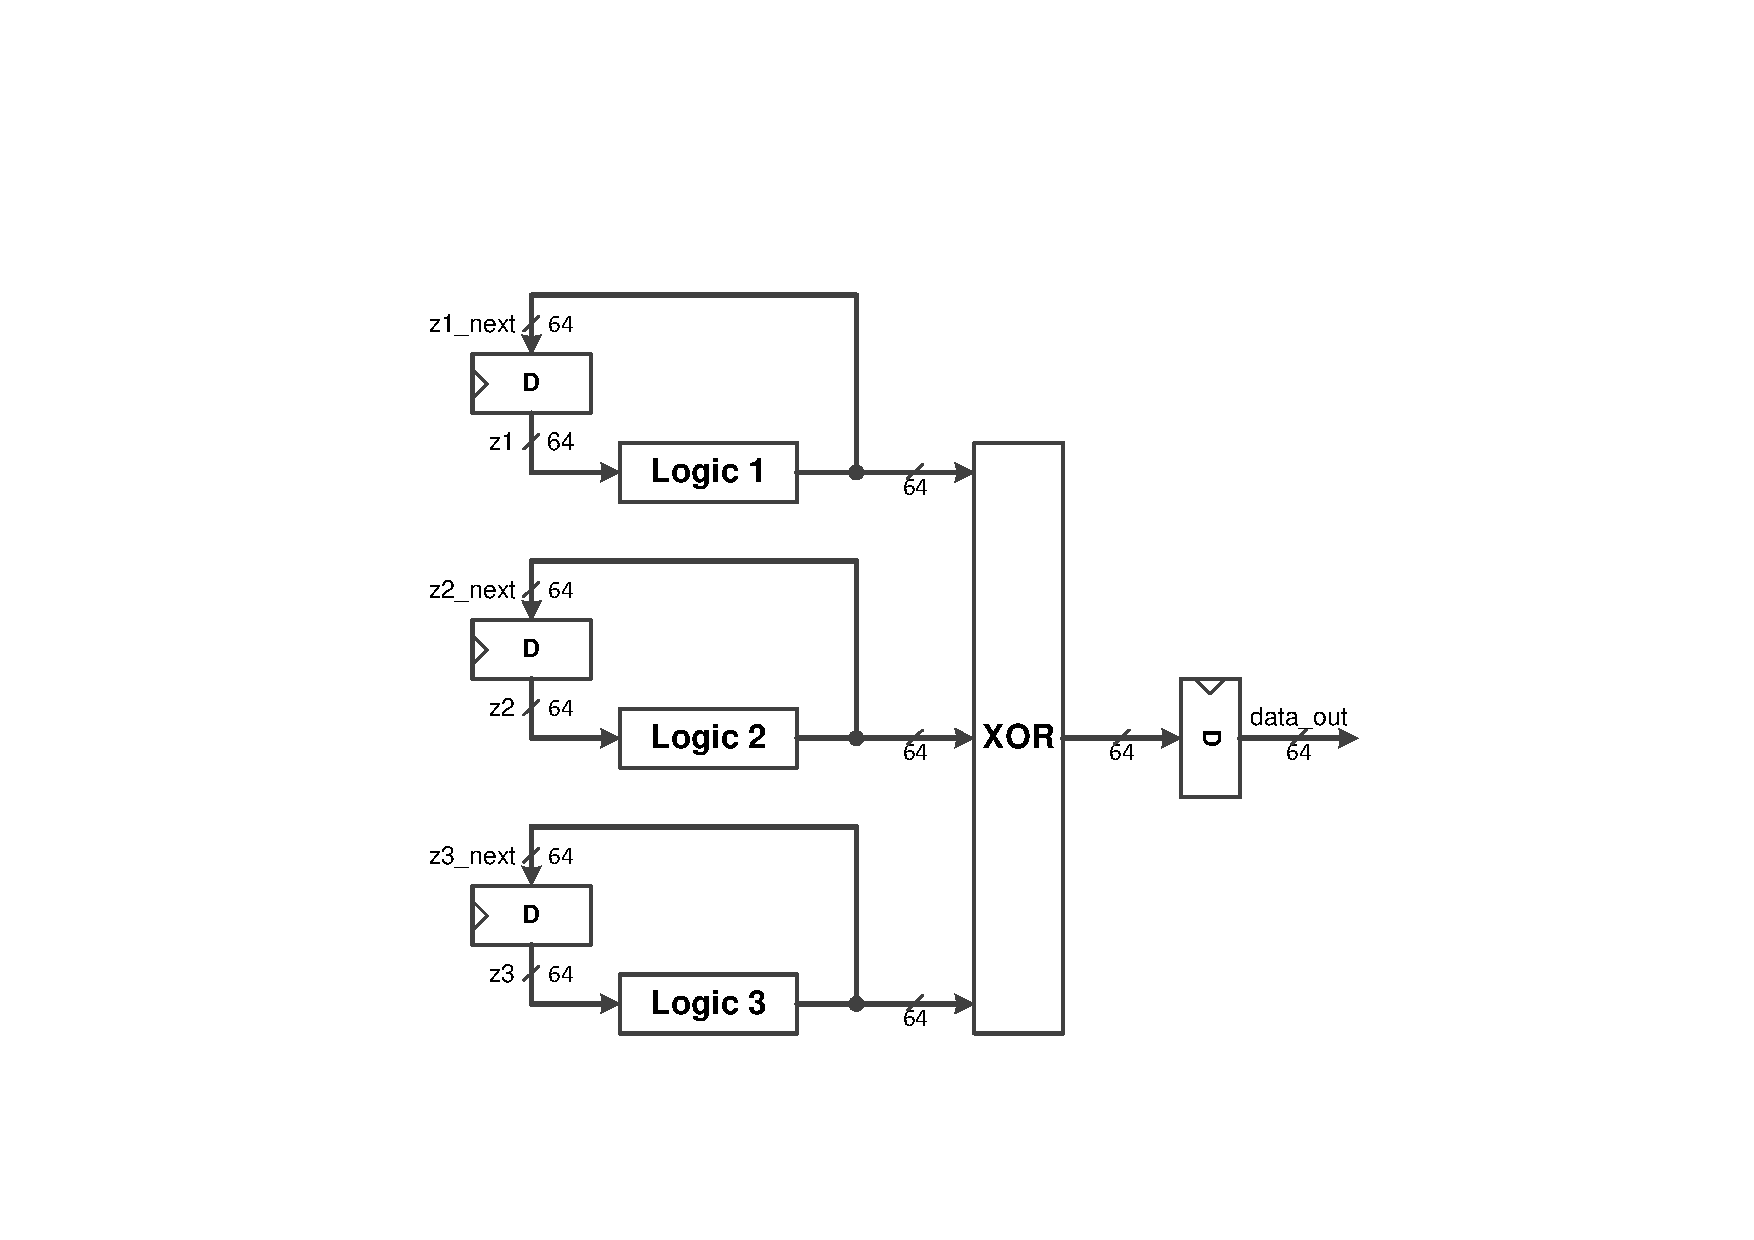
\includegraphics[scale=0.7,angle=270]{ctgarch.pdf}
\caption{Architecture of CTG.}
\label{fig:ctgarch}
\end{figure}

The initial values of registers $z_1$, $z_2$ and $z_3$ are precalculated.
And combinatorial logic for each branch is
(symbol $\oplus$ denotes the logical exclusive-or operator)
\begin{align}
    z_{1,\,\text{next}} &= \left\{ z_1[39:1], z_1[58:34] \oplus z_1[63:39] \right\}; \\
    z_{2,\,\text{next}} &= \left\{ z_2[50:6], z_2[44:26] \oplus z_2[63:45] \right\}; \\
    z_{3,\,\text{next}} &= \left\{ z_3[56:9], z_3[39:24] \oplus z_3[63:48] \right\}.
\end{align}

\subsubsection{ICDF}
The architecture of \textsf{CTG} is depicted in Figure \ref{fig:icdfarch}.
For simplicity the control signals and registers are not presented.
\begin{figure}[!htbp]
\centering
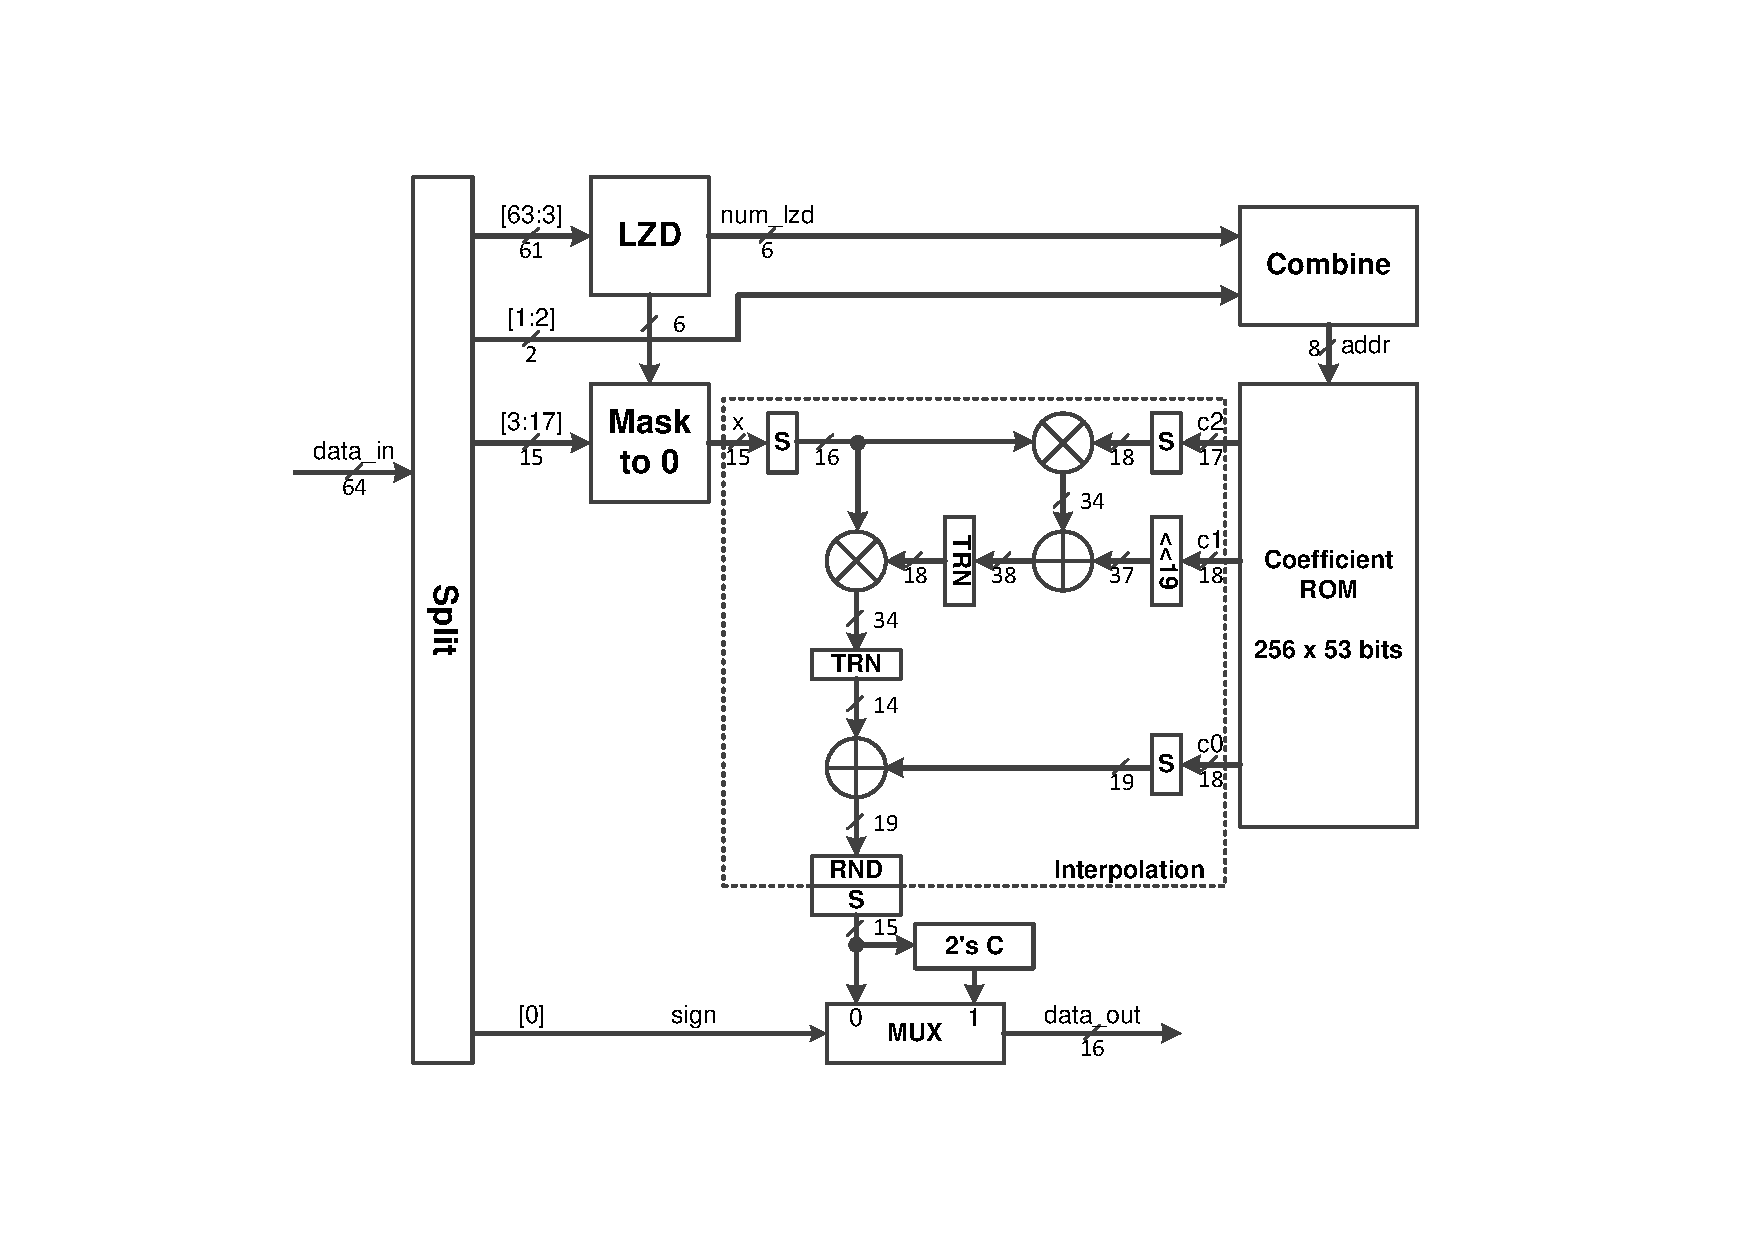
\includegraphics[scale=0.55,angle=270]{icdfarch.pdf}
\caption{Architecture of ICDF.}
\label{fig:icdfarch}
\end{figure}

Where submodule \textsf{S} is sign bit extension,
\textsf{TRN} is data truncation, and \textsf{RND} is data round.
All multipliers and adders are signed operation.

Submodule \textsf{LZD} is to count number of leading zeros of 61-bit number.
Here we choose the methodology proposed in \cite{oklobdzija}.
The architecture of \textsf{LZD} is shown in Figure \ref{fig:lzdarch}.
\begin{figure}[!htbp]
\centering
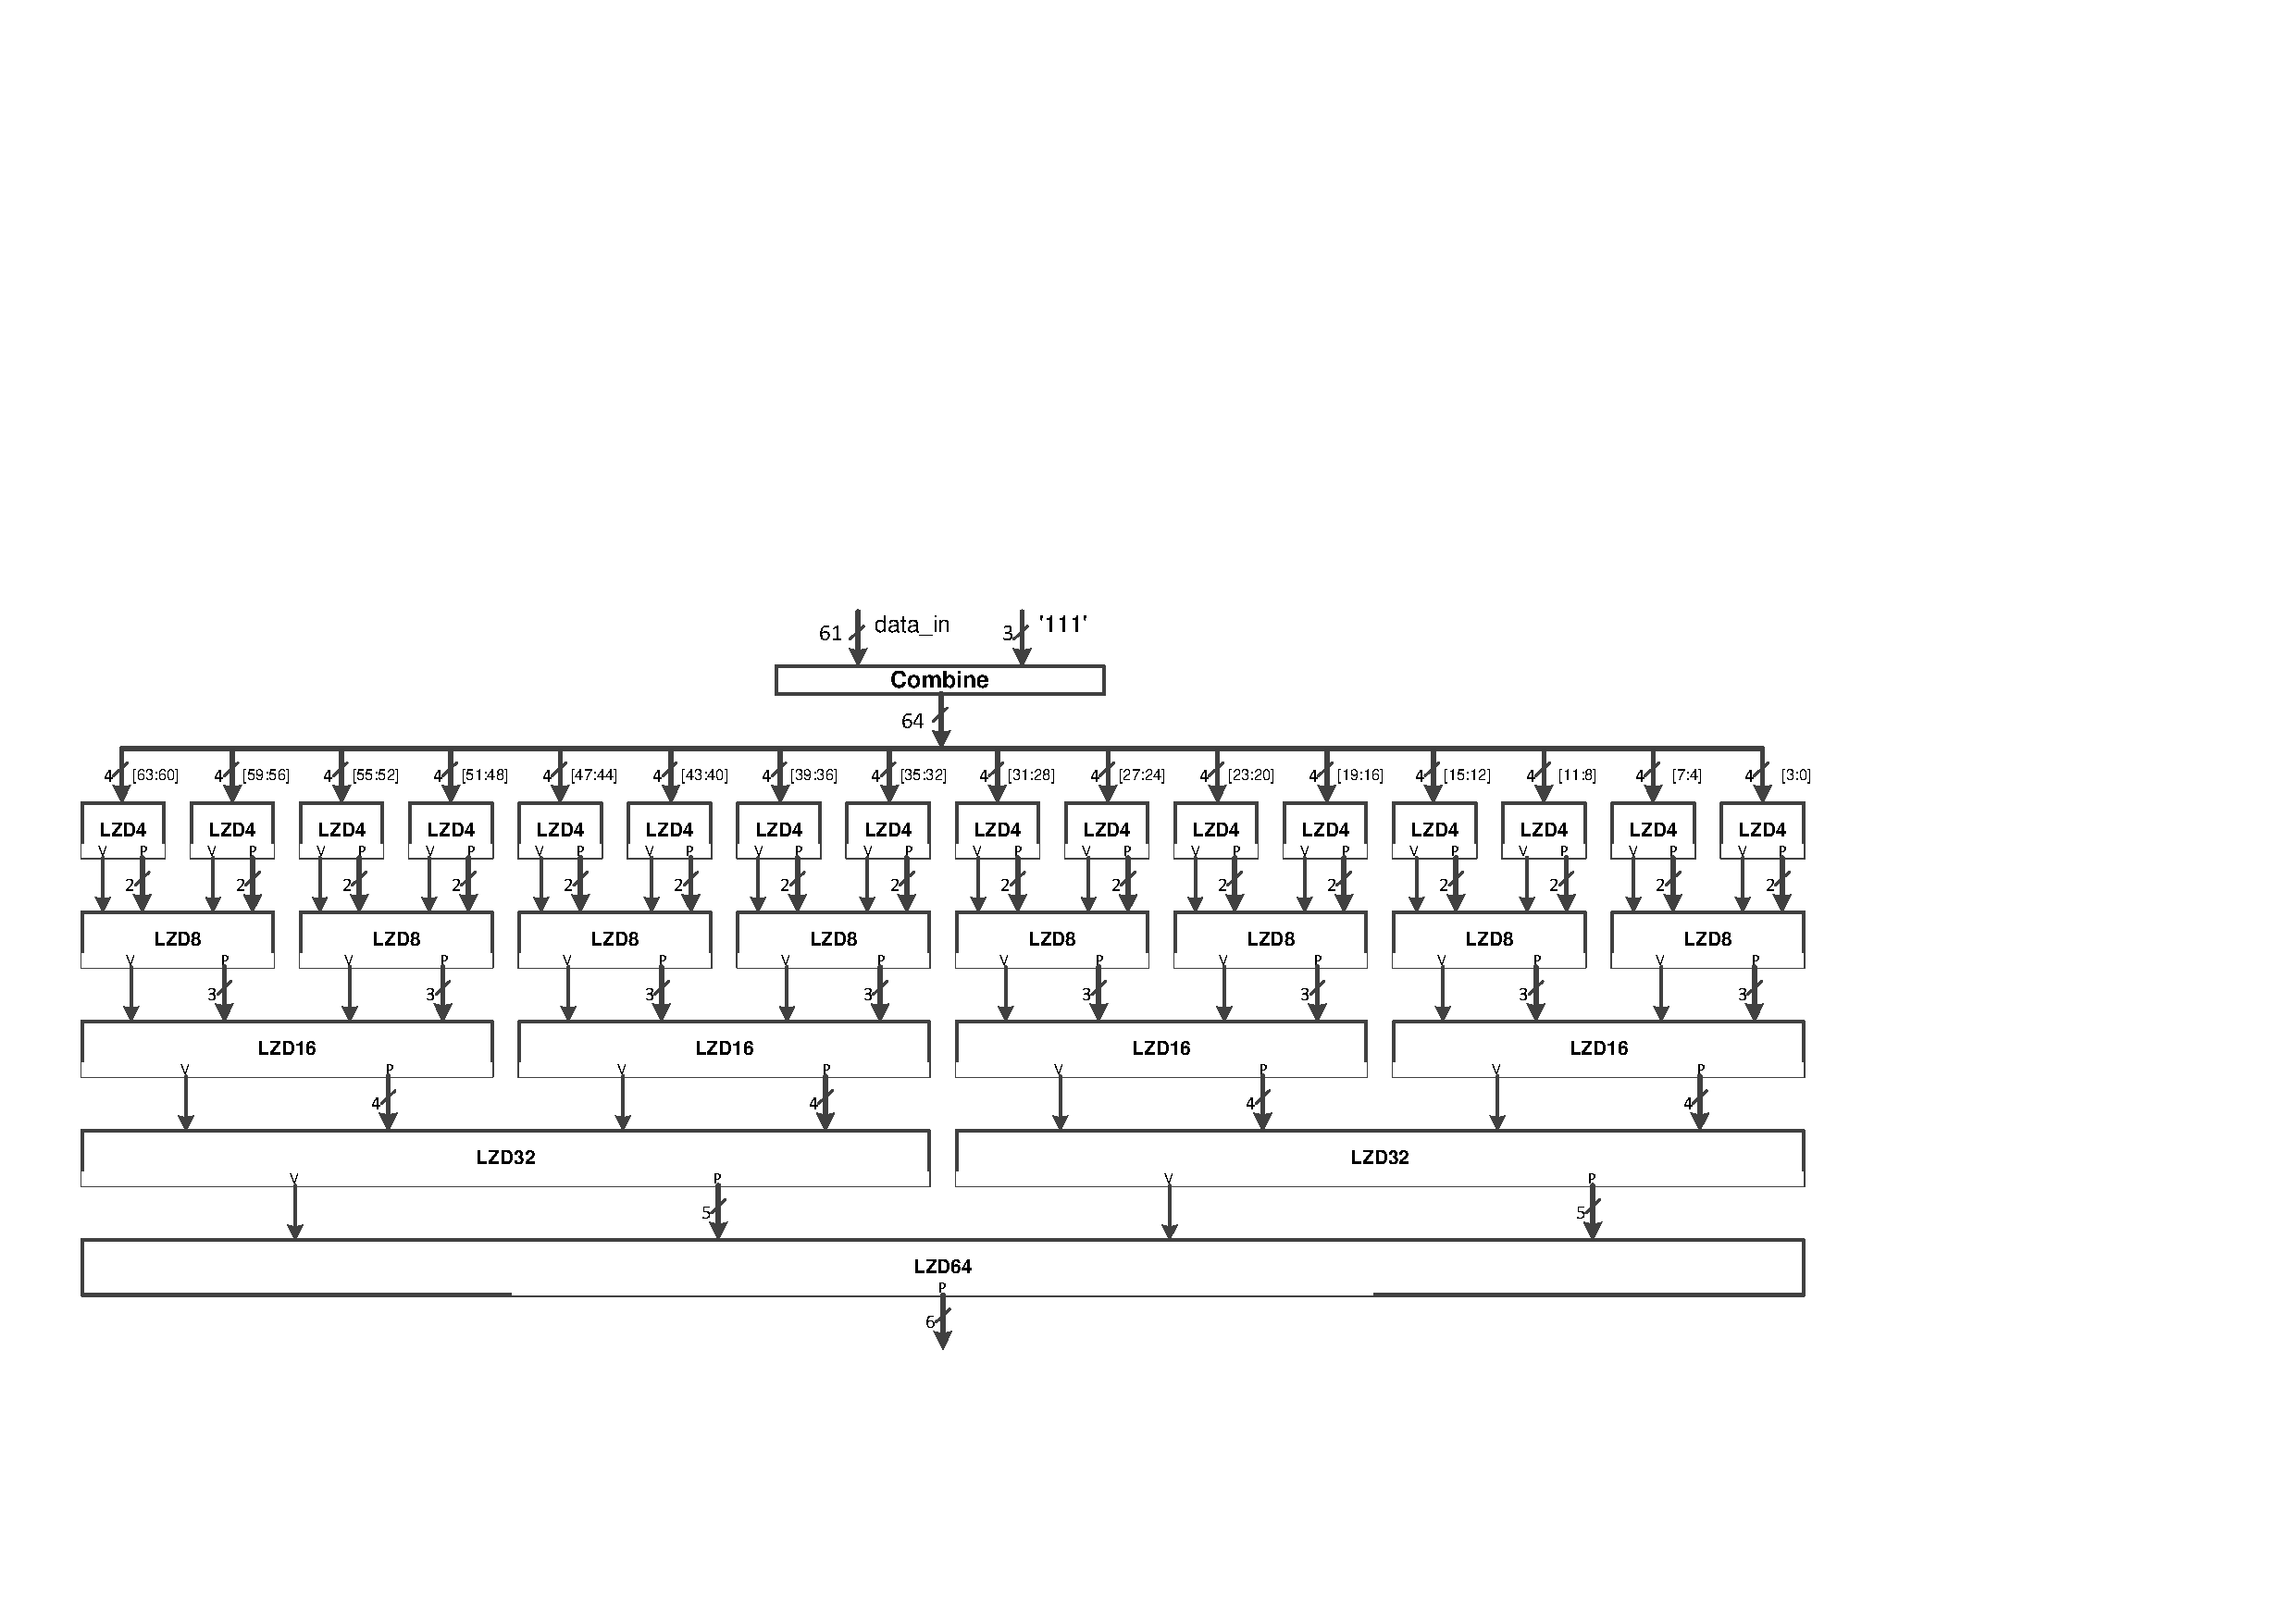
\includegraphics[scale=0.35,angle=270]{lzdarch.pdf}
\caption{Architecture of LZD.}
\label{fig:lzdarch}
\end{figure}

Where the logic of \textsf{LZD4} is as below
\begin{align}
    V &= d[0] | d[1] | d[2] | d[3], \\
    P &= \left\{ \overline{d[2] | d[3]},
        ((d[2] | d[3]) \,?\, \overline{d[3]} : \overline{d[1]} \right\}.
\end{align}
And the logic of \textsf{LZD8} is
\begin{align}
    V &= V[0] | V[1], \\
    P &= \left\{ \overline{V[1]}, ((V[1]) \,?\, P[1] : P[0]) \right\}.
\end{align}
And so on. Note that in the last level \textsf{LZD64} only \textsf{P} is used.

\subsection{Timing}
The typical timing diagram is in Figure \ref{fig:coretiming}.
\begin{figure}[!htbp]
\centering
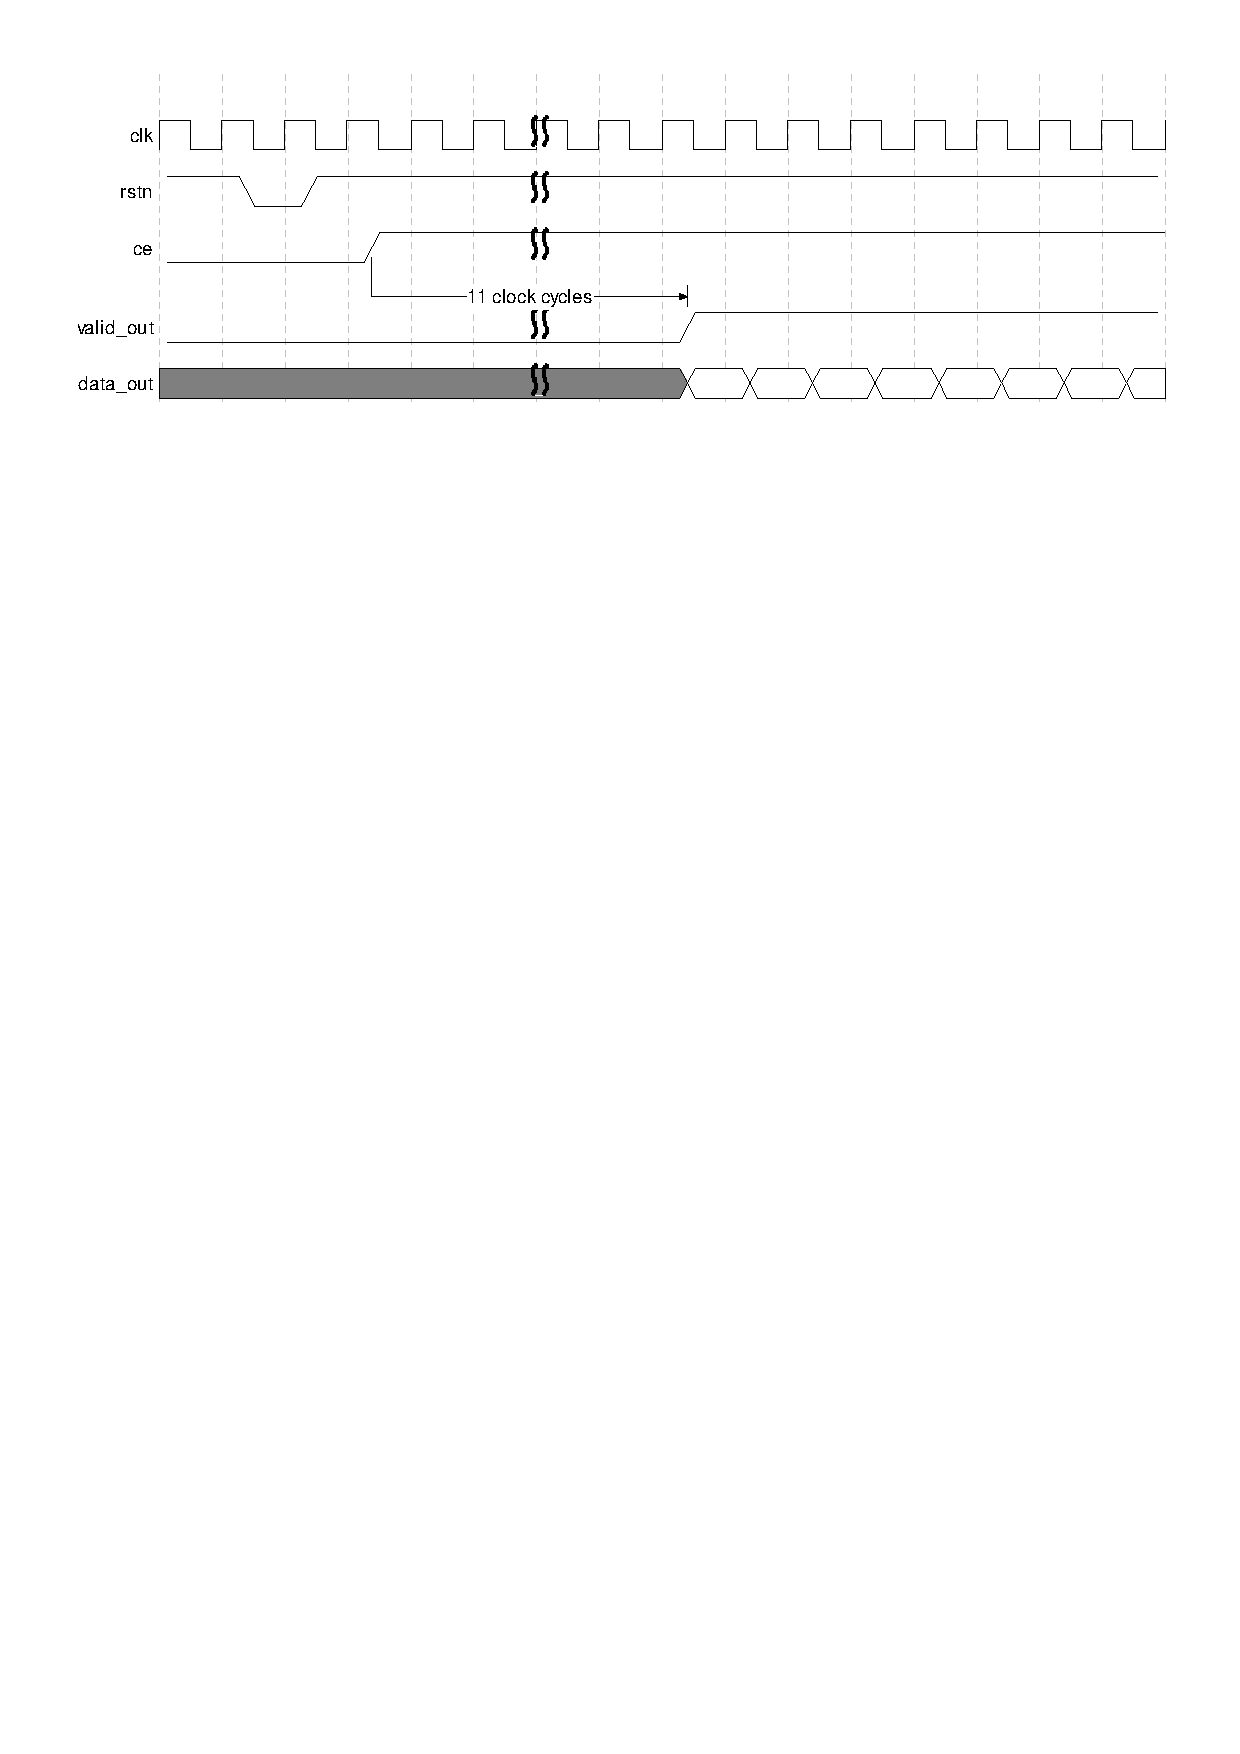
\includegraphics[scale=0.6]{coretiming.pdf}
\caption{Core timing diagram.}
\label{fig:coretiming}
\end{figure}

The signal \textsf{valid\_out} asserts after 11 clock cycles
when signal \textsf{ce} asserts.
If \textsf{ce} is tied high, \textsf{data\_out} is output every clock.


\section{C/MATLAB Model}

\subsection{C codes}
We use C codes to build the functional model.
The file names and their descriptions are listed in Table \ref{tbl:ccode} below.
\begin{table}[!htbp]
\centering
\caption{C codes list.}
\label{tbl:ccode}
\begin{tabular}{cp{8cm}}
    \addlinespace
    \toprule

    \textbf{File Name} & \textbf{Description} \\

    \midrule

    \textsf{taus176.h} &
        Header file for maximally equidistributed combined Tausworthe generator \\
    \textsf{taus176.c} &
        Implementation file for maximally equidistributed combined Tausworthe generator \\
    \textsf{icdf.h} &
        Header file for piecewise polynomial approximation of inverse of
        the normal cumulative distribution function \\
    \textsf{icdf.c} &
        Implementation file for piecewise polynomial approximation of inverse of
        the normal cumulative distribution function \\

    \bottomrule
\end{tabular}
\end{table}

These codes are also used as C MEX codes in MATLAB model (See next subsection).

\subsection{C MEX and MATLAB codes}
To accelerate MATLAB simulation speed, C MEX method is used.
The file names and their descriptions are listed in Table \ref{tbl:cmex} below.
\begin{table}[!htbp]
\centering
\caption{C MEX/MATLAB codes list.}
\label{tbl:cmex}
\begin{tabular}{cp{8cm}}
    \addlinespace
    \toprule

    \textbf{File Name} & \textbf{Description} \\

    \midrule

    \textsf{ctg\_seed.c} &
        C MEX file for generate Combined Tausworthe Generator seed \\
    \textsf{ctg\_seed.m} &
        MATLAB helper file for \texttt{ctg\_seed} function \\
    \textsf{ctg\_gen.c} &
        C MEX file for generate Combined Tausworthe number \\
    \textsf{ctg\_gen.m} &
        MATLAB helper file for \texttt{ctg\_gen} function \\
    \textsf{icdf\_gen.c} &
        C MEX file for generate inverse of the normal cumulative distribution function \\
    \textsf{icdf\_gen.m} &
        MATLAB helper file for \texttt{icdf\_gen} function \\
    \textsf{build\_mex.m} &
        Build above C MEX files \\
    \textsf{test\_gng.m} &
        Test Gaussian noise generator \\

    \bottomrule
\end{tabular}
\end{table}

Note that 64-bit integer data type is used in C MEX file,
and VC++ should be used as compile in MATLAB \texttt{mex setup}.
Typical versions are MATLAB R2011b and Visual C++ 2010.


\section{Synthesis}

\subsection{Xilinx FPGA}
FPGA Device is Virtex-6 XC6VLX240T-2ff1156 and
implementation tool is Xilinx ISE 14.7.
Results are shown in table \ref{tbl:impxil}, and are slightly better than \cite{dicomlab}.
\begin{table}[!htbp]
\centering
\caption{Implementation results (place and route) for Xilinx FPGA.}
\label{tbl:impxil}
\begin{tabular}{cc}
    \addlinespace
    \toprule

    \textbf{Parameter} & \textbf{Value} \\

    \midrule

    Number of occupied Slices & 97 \\
    Number of RAMB36E1 & 1 \\
    Number of DSP48E1s & 2 \\
    Maximum frequency & \SI{311.8}{\milli\watt} \\

    \bottomrule
\end{tabular}
\end{table}

\subsection{Altera FPGA}
FPGA Device is Stratix IV GX EP4SGX230KF40C3 and
implementation tool is Altera Quartus II 11.1.
Results are shown in table \ref{tbl:impalt}, and are slightly better than \cite{dicomlab}.
\begin{table}[!htbp]
\centering
\caption{Implementation results (place and route) for Altera FPGA.}
\label{tbl:impalt}
\begin{tabular}{cc}
    \addlinespace
    \toprule

    \textbf{Parameter} & \textbf{Value} \\

    \midrule

    Total LABs & 34 \\
    M9K blocks & 2 \\
    DSP block 18-bit elements & 4 \\
    Maximum frequency & \SI{376.8}{\milli\watt} \\

    \bottomrule
\end{tabular}
\end{table}

\subsection{ASIC}
ASIC technology library is SMIC 55nm LL and
synthesis tool is Synopsys Design Compiler 2012.06-SP3.
Results are shown in table \ref{tbl:impsmic}.
\begin{table}[!htbp]
\centering
\caption{Implementation results for SMIC library.}
\label{tbl:impsmic}
\begin{tabular}{cc}
    \addlinespace
    \toprule

    \textbf{Parameter} & \textbf{Value} \\

    \midrule

    Area & \SI{16739.52}{\square\micro\meter} \\
    Equivalent gates & \num{13078} \\
    Target frequency & \SI{400.0}{\mega\hertz} \\
    Power & \SI{4.2133}{\milli\watt} \\

    \bottomrule
\end{tabular}
\end{table}

The smallest area (\SI{1.28}{\square\micro\meter}) of an NAND2 gate is used as
the base in equivalent gates calculation.
Notice that the results are not the best due to
the core is not specially optimized for ASIC.


\section{Simulation}

\subsection{Test Bench}
To verify the correction of the core, a SystemVerilog code
(\textsf{tb\_gng.sv}) is written to do it.
First, we use \texttt{ctg\_seed(1)} command in MATLAB to generate
the core parameters \textsf{INIT\_Z1}, \textsf{INIT\_Z2} and
\textsf{INIT\_Z3}, which are just the default parameters in code \textsf{gng.v}.

The design gng is instantiated as a design under test (DUT) in test bench.
The basic function of test bench is:
generate \num{e6} active signal \textsf{ce} to the DUT,
and record its output data to a data file (\textsf{gng\_data\_out.txt}).

\subsection{Simulation Result}
By running the simulation script file run.do in ModelSim,
the result data file \textsf{gng\-\_data\-\_out.txt} can be generated.
Meanwhile by running the m file \textsf{test\_gng.m} in MATLAB,
the variable \texttt{x} is gotten.
Then Import the data in \textsf{gng\_data\_out.txt} into MATLAB
and compare it with \texttt{x}.
The comparison result should be all equal,
which means the function of RTL exactly matching that of MATLAB model.


\section{Revision History}
\begin{center}
\begin{tabular}{cccp{4cm}}
    \toprule

    \textbf{Revision} & \textbf{Date} & \textbf{Author}
        & \textbf{Description} \\

    \midrule

    \oldstylenums{0.1} & \oldstylenums{2014/8/4} & Guangxi Liu
        & First Draft \\
    \oldstylenums{1.0} & \oldstylenums{2015/1/29} & Guangxi Liu
        & Revision 1.0 \\
    \oldstylenums{1.1} & \oldstylenums{2016/7/27} & Guangxi Liu
        & Rewrite using \LaTeX \\

    \bottomrule
\end{tabular}
\end{center}

\clearpage


% References
\bibliography{gng}


\end{document}
